\documentclass{article}[12pt]

% useful packages
\usepackage{fullpage}
\usepackage{amsmath,amssymb,amsthm,amsfonts}
\usepackage{graphicx}
\usepackage{enumerate}
\usepackage{algorithm,algorithmic}
\usepackage{xcolor}
\usepackage{bbm}
\usepackage{url}
\usepackage{caption,subcaption}

% theorem type environments
\newtheorem{thm}{Theorem}
\newtheorem{prop}{Proposition}
\newtheorem{lemma}{Lemma}
\newtheorem{cor}{Corollary}
\newtheorem{defn}{Definition}
\newtheorem{assump}{Assumption}
\newtheorem{example}{Example}
\newtheorem{conjecture}{Conjecture}

% frequently used symbols
\newcommand{\bE}{\mathbb{E}}
\newcommand{\bP}{\mathbb{P}}
\newcommand{\bQ}{\mathbb{Q}}
\newcommand{\bR}{\mathbb{R}}
\newcommand{\bS}{\mathbb{S}}
\newcommand{\bN}{\mathbb{N}}
\newcommand{\bZ}{\mathbb{Z}}
\newcommand{\sC}{{\mathcal C}} 
\newcommand{\sD}{{\mathcal D}} 
\newcommand{\sE}{{\mathcal E}} 
\newcommand{\sF}{{\mathcal F}} 
\newcommand{\sL}{{\mathcal L}} 
\newcommand{\sH}{{\mathcal H}} 
\newcommand{\sN}{{\mathcal N}} 
\newcommand{\sO}{{\mathcal O}} 
\newcommand{\sP}{{\mathcal P}} 
\newcommand{\sR}{{\mathcal R}} 
\newcommand{\sS}{{\mathcal S}}
\newcommand{\sU}{{\mathcal U}} 
\newcommand{\sX}{{\mathcal X}} 
\newcommand{\sY}{{\mathcal Y}} 
\newcommand{\sZ}{{\mathcal Z}}

% operators
\newcommand{\sign}{\mathop{\mathrm{sign}}}
\newcommand{\supp}{\mathop{\mathrm{supp}}} % support
\newcommand{\argmin}{\operatornamewithlimits{arg\ min}}
\newcommand{\argmax}{\operatornamewithlimits{arg\ max}}
\newcommand{\dist}{\operatorname{dist}}
\newcommand{\tr}{\text{tr}}
\newcommand{\vecop}{\text{vec}}
\newcommand{\st}{\operatorname{s.t.}}
\newcommand{\cut}{\setminus}
\newcommand{\ra}{\rightarrow}
\newcommand{\ind}[1]{\mathbbm{1}\left\{#1\right\}} 
\newcommand{\given}{\ | \ }

% grouping operators
\newcommand{\brac}[1]{\left[#1\right]}
\newcommand{\set}[1]{\left\{#1\right\}}
\newcommand{\abs}[1]{\left\lvert #1 \right\rvert}
\newcommand{\paren}[1]{\left(#1\right)}
\newcommand{\norm}[1]{\left\|#1\right\|}
\newcommand{\ip}[2]{\left\langle #1,#2 \right\rangle}

% code commands
\newcommand{\matlab}{\textsc{Matlab }}
\newcommand{\algname}[1]{\textnormal{\textsc{#1}}}

% header command
\newcommand{\homework}[4]{
    \pagestyle{myheadings}
    \thispagestyle{plain}
    \newpage
    \setcounter{page}{1}
    \setlength{\headsep}{10mm}
    \noindent
    \begin{center}
    \framebox{
        \vbox{\vspace{2mm}
            \hbox to 6.28in { {\bf STAT 672: Statistical Learning II
            \hfill Winter 2020} }
        \vspace{4mm}
        \hbox to 6.28in { {\Large \hfill Homework #1 \hfill} }
        \vspace{2mm}
        \hbox to 6.28in { \Large \hfill Due: #2 \hfill }
        \vspace{2mm}
        \hbox to 6.28in { {\it Student Name: #3} \hfill {\it Professor Name: #4}}
        \vspace{2mm}}
   }
   \end{center}
   \markboth{Homework #1}{Homework #1}
   \vspace*{4mm}
}

\begin{document}
\homework{2}{February 5th, 2020}{Ethan Lew}{Bruno Jedynak}
\section{Kernel centering}
Let $\mathcal{X}$ be a non empty set, $K$ a kernel over $\mathcal{X}$ and $H$ the RKHS with kernel $K$. Let $x_1,\ldots,x_n$, be $n$ points in $\mathcal{X}$. 

Let $K_c$ like ``K centered\rq\rq{} be another kernel over $\mathcal{X}$ defined by 
\begin{equation}
K_c(x,y)=\langle K(.,x)- \bar{f}(.), K(.,y)-\bar{f}(.)\rangle_H \mbox{, with } \bar{f}(.)=\frac{1}{n}\sum_{i=1}^n K(.,x_i)
\end{equation}
\begin{enumerate}
\item Verify that $K_c$ is a positive definite kernel;

	\textbf{Solution:} A kernel $K$ is said to be positive definite if it satisfies the condition \begin{equation}
		\sum^{m}_{i=1} \sum^{m}_{j=1} \alpha_i \alpha_j K(x_i, x_j) \ge 0,  		
\end{equation}
for $\alpha_1,...,\alpha_m \in \mathbb R$, $x_1,...,x_m \in \mathcal X$. Manipulate the expression, 
\begin{equation}
	\begin{aligned}
		\sum^{m}_{i=1} \sum^{m}_{j=1} \alpha_i \alpha_j  &\langle K(.,x_i)- \bar{f}(.), K(.,x_j)-\bar{f}(.)\rangle_H \\ 
		&= \sum^{m}_{i=1} \sum^{m}_{j=1} \alpha_i \alpha_j K(x_i, x_j) - 2 \sum^{m}_{i=1} \sum^{m}_{j=1} \alpha_i \alpha_j \bar f(x_i)  + \sum^{m}_{i=1} \sum^{m}_{j=1} \alpha_i \alpha_j || \bar f ||_{\mathcal H}^2 \\
		&= \left| \left| \sum^{m}_{i=1} \alpha_i K(., x_i)  \right| \right|^2_{\mathcal H} + \left| \left| \sum^{m}_{i=1} \alpha_i f  \right| \right|^2_{\mathcal H} - 2 \langle \sum^{m}_{i=1} \alpha_i K(., x_i), \sum^{m}_{i=1} \alpha_i \bar f  \rangle_{\mathcal H}  
	\end{aligned}
\end{equation}
As,
\begin{equation}
	 \left| \left| \sum^{m}_{i=1} \alpha_i K(., x_i)  \right| \right|^2_{\mathcal H} + \left| \left| \sum^{m}_{i=1} \alpha_i f  \right| \right|^2_{\mathcal H} \ge  2 \langle \sum^{m}_{i=1} \alpha_i K(., x_i), \sum^{m}_{i=1} \alpha_i \bar f  \rangle_{\mathcal H}, 
\end{equation}
$K_c$ meets the positive definite condition.

Alternatively, the PD condition can be seen as the norm of a difference,
\begin{equation}
	\begin{aligned}
		\sum^{m}_{i=1} \sum^{m}_{j=1} \alpha_i \alpha_j \langle K(., x_i) - \bar f, K(., x_j) - \bar f \rangle &= \langle \sum^{m}_{i=1} \alpha_i K(x_i, .), \sum^{m}_{i=1} \alpha_i K(x_i,.)   \rangle \\
														       &= \left| \left| \sum^{m}_{i=1} \alpha_i K(x_i, .)  \right| \right| \\
														       &\ge 0.
	\end{aligned}

\end{equation}

	
Let $H_c$ be the RKHS with reproducing kernel $H_c$. 
\item (**) Verify that for any $f \in H_c$, 
\begin{equation}
\frac{1}{n} \sum_{i=1}^n f(x_i)=0
\end{equation}

\textbf{Solution:} Recall the reproducing property,
\begin{equation}
	f(x) = \langle f, K(., x) \rangle_{\mathcal H}.
\end{equation}
Manipulate the given expression,
\begin{equation}
	\begin{aligned}
		\frac{1}{n} \sum^{n}_{i=1} f(x_i) &= \frac{1}{n} \sum^{n}_{i=1} \langle K_c(., x_i), f \rangle_{\mathcal H}  \\
	  &= \langle \frac{1}{n} \sum^{n}_{i=1} K_c(., x_i), f  \rangle \\
	  &= \langle \frac{1}{n} \sum^{n}_{i=1} \left( K(., x_i) - \bar{f} \right), f   \rangle_{\mathcal H} \\
	  &= \langle \bar{f} -\bar{f}, f \rangle_{\mathcal H}\\
	  &= 0. \\
	\end{aligned}
\end{equation}



In homework 1, you have learned to sample functions from a RKHS with kernel $K$ over the set $\mathcal{X}=\{-m,\ldots,m\}$ according to the probability 
\begin{equation}
p(f)=Ce^{-\frac{||f||^2}{2}}
\end{equation} 
Here, you are asked to do the same thing but over the RKHS of a centered kernel $K_c$. Specifically, choose  $m=10$, $n=11$, $x_1=-10,x_2=-9,\ldots,x_{11}=0$. 
\item (**) Write $K_c$ in term of $K$ using matrix operations. 

	\textbf{Solution:} Perform the substitution $\bar f (.) = \frac{1}{n} \sum^{n}_{i=1} K(., x_i)$,
	\begin{equation}
		\begin{aligned}
			\langle K(., x) - \bar f(.), K(., y) - \bar f(.) \rangle_{\mathcal H} &= \langle K(x,y) - \frac{1}{n} \sum^{n}_{i=1} K(., x_i) , K(., y) - \frac{1}{n} \sum^{n}_{i=1} K(., x_i)  \rangle_{\mathcal H} \\
											      &= K(x,y) - \frac{1}{n} \sum^{n}_{i=1} K(x, x_i) - \frac{1}{n} \sum^{n}_{i=1} K(y, x_i) + \frac{1}{n^2} \sum^{n}_{i=1} \sum^{n}_{j=1} K(x_i, x_j).        
		\end{aligned}
	\end{equation}
	Now prepare for matrix multiplication form by defining the notation of $ij$ entry of the matrix $K$,
\begin{equation}
	[K]_{ij} = K(x_i, x_j).
\end{equation}
This allows writing the expression as
\begin{equation}
	K_c (x_i, x_j) = K_{ij} - \frac{1}{n} \sum^{n}_{l=1} K_{li} - \frac{1}{n} \sum^{n}_{l=1} K_{lj} + \frac{1}{n^2} \sum^{n}_{l=1} \sum^{n}_{k=1} K_{lk}.
\end{equation}
Summing the columns is equvalent to multiplying the matrix $K$ by a vectors of ones, $\mathbbm 1_n$,
\begin{equation}
	K_c(x_i, x_j) = K_{ij} - \frac{1}{n} K^T_i \mathbbm l_n - \frac{1}{n} K^T_j \mathbbm l_n + \frac{1}{n^2} \mathbbm l_n^T K \mathbbm l_n.   
\end{equation}
For the entire matrix $K_c$, the entries can be found by the operation
\begin{equation}
	K_c = K - UK -KU + UKU,
\end{equation}
where 
\begin{equation}
	U \in \mathbb R^{n \times n}, \quad [U]_{ij} = \frac{1}{n}. 
\end{equation}
Factoring,
\begin{equation}
	K_c = (I-U)K(I-U).
\end{equation}

\item Choose the Gaussian kernel with $\tau=10$, and show 10 samples. Check that for each curve $f$, 
\begin{equation}
\frac{1}{11}\sum_{i=-10}^0 f(i)=0
\end{equation}
up to numerical errors.

\textbf{Solution:} The code was shown to be within numerical error of zero. See Figure \ref{fig:gauss_prob1} for the samples plot.

\begin{figure}
	\centering
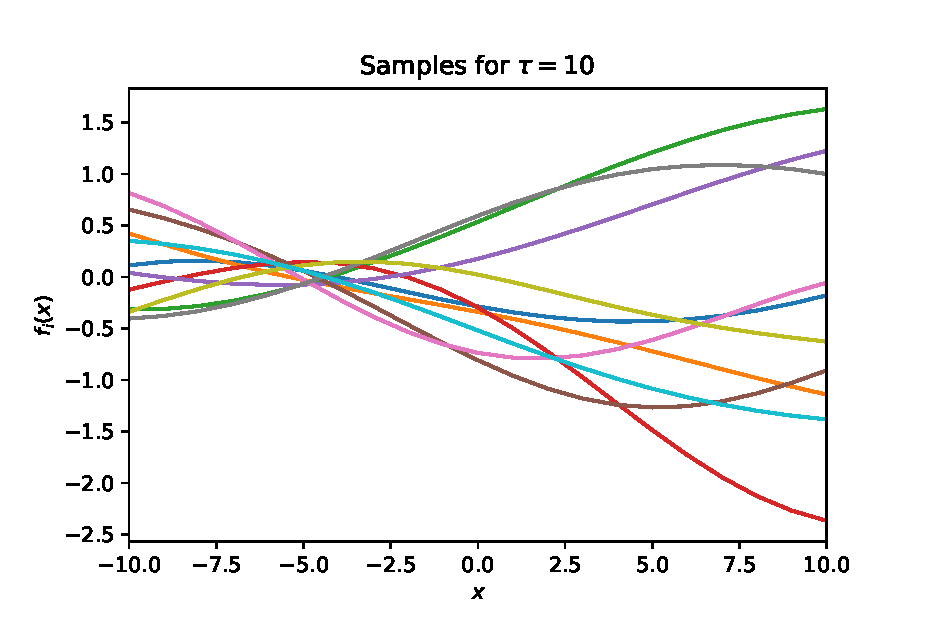
\includegraphics[width=0.5\textwidth]{./img/problem1.eps}
\caption{\label{fig:gauss_prob1} Samples of the Gaussian Process for the Kernel}
\end{figure}

%\begin{figure}
%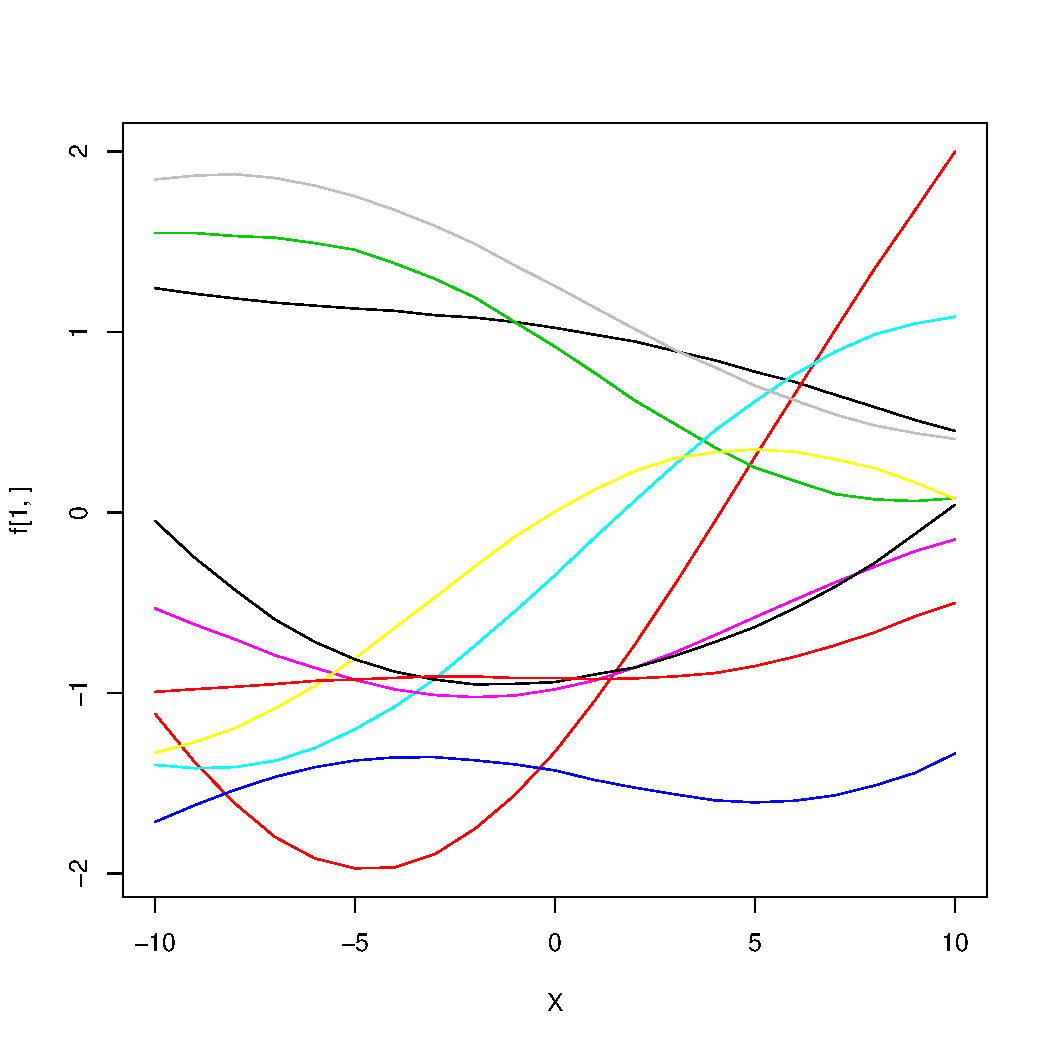
\includegraphics[width=0.5\textwidth]{Gauss.pdf}
%\caption{\label{fig:Gauss_constraint}Example of 10 samples of \lq{}\rq{}functions\rq\rq{} of the RKHS over $\{-10,\ldots,10\}$ with the Gaussian kernel, $\tau=10$ under the centering constraint $\frac{1}{11}\sum_{i=-10}^0 f(i)=0$}
%\end{figure}
\end{enumerate}

\section{Kernel PCA}
$\mathcal{X}$ a non empty set, $x_1,\ldots,x_n \in \mathcal{X}$, $K$ a centered kernel, that is, starting with a kernel $G$ over $\mathcal{X}$, 
  \begin{equation}
K(x,y)=\langle G(.,x)- \bar{f}, G(.,y)-\bar{f}\rangle_H \mbox{, with } \bar{f}=\frac{1}{n}\sum_{i=1}^n G(.,x_i)
\end{equation}
Assume for simplicity that $K$ is full rank. Notate $\lambda_1 \geq \lambda_2 \geq \ldots \geq \lambda_n>0$ the e-values and $u_1,\ldots,u_n$ the corresponding e-vectors. 
We have seen in class that the principal directions $f_1,\ldots,f_n$ are 
\begin{equation}
f_i=\sum_{j=1}^n \alpha_{ij} K(.,x_j), \mbox{ with } \alpha_i = \lambda_i^{-\frac{1}{2}}u_i
\end{equation}
\begin{enumerate}
\item verify that 
\begin{equation}
\langle f_i,f_k \rangle_H=\delta_{ik}
\end{equation}
where $\delta_{ik}=1$ if $i=k$ and $\delta_{ik}=0$ if $i \not = k$. 

\textbf{Solution:} Substitute the full expression for $f_i$,
\begin{equation}
	\begin{aligned}
	\langle f_i, f_k \rangle_{H} &= \langle \sum^{n}_{j=1} \lambda^{-1/2} u_{ij} K(., x_j), \sum^{n}_{l=1} \lambda^{-1/2}_k u_{kl} K(., x_l)   \rangle_H \\
				     &= \sum^{n}_{j=1} \sum^{n}_{l=1} \lambda_k^{-1/2} \lambda_i^{-1/2} u_{ij} u_{kl} \langle K(., x_j), K(., x_l) \rangle_H. \\  
	\end{aligned}
\end{equation}
Define a matrix $K \in \mathbb R^{n \times n}$,
\begin{equation}
	[K]_{ij} = K(x_i, x_j).
\end{equation}
This permits the form,
\begin{equation}
	\begin{aligned}
		\left( \lambda_i^{-1/2} u_i^T \right) K \left( \lambda_k^{-1/2} u_k \right) = \left( \lambda_i^{-1/2} \lambda_k^{-1/2} \right) u_i^T K u_k.
	\end{aligned}
\end{equation}
As $K$ is positive definite, it permits eigendecomposition, 
\begin{equation}
	K =  U\Lambda U^T,\quad UU^T = I, \quad [\Lambda]_{ij} = \begin{cases} \lambda_i \quad i = j \\ 0 \quad i \ne j \end{cases}.
\end{equation}
Substitute the decomposition,
\begin{equation}
	\begin{aligned}
		\left( \lambda_i^{-1/2} \lambda_k^{-1/2} \right) \left(u_i^T U \right) \Lambda \left( U^T u_k \right) &=  \left( \lambda_i^{-1/2} \lambda_k^{-1/2} \right) e_i \Lambda e_j \\
	&= \begin{cases}
		1 \quad i = j \\
		0 \quad i \ne j \\
	\end{cases}\\
	&= \delta_{ij}.
	\end{aligned}
\end{equation}





\item Show that the orthogonal projection of any $f \in H$, the RKHS with kernel $K$ onto 
\begin{equation}
	V=\operatorname{span}\left(\{f_1,\ldots,f_n\}\right)
\end{equation} is 
\begin{equation}
\pi_v(f)=\langle f,f_1\rangle_H f_1+\ldots,\langle f,f_n\rangle_H f_n
\end{equation}

\textbf{Solution:} A function $\pi_V : H \rightarrow V$ is an orthogonal projection if it satisfies two properties,
\begin{enumerate}[(i)]
	\item \[
			\pi_V(f) \in V
	\]
	\item \[
			\langle f- \pi_V(f), g \rangle_H = 0, \forall g \in V
	\] 
\end{enumerate}
$V$ can be defined as,
\begin{equation}
	V = \left\{ f: f = \sum^{n}_{i=1} \alpha_i f_i, \alpha_i \in \mathbb R   \right\}.
\end{equation}
It is clear, then, that $\pi_V(f)$ is in $V$ as $\langle f, f_i \rangle_H$ can be set as $\alpha_i$, satisfying the first condition.

Next, recall that all $g \in V$ can take the form,
\begin{equation}
	g = \sum^{n}_{i=1} \beta_i f_i. 
\end{equation}
Substitute that into the second condition,
\begin{equation}
	\begin{aligned}
		\langle f - \pi_V(f), g \rangle &= \langle f - \sum^{n}_{i=1} \langle f, f_i \rangle f_i, \sum^{n}_{i=1} \beta_i f_i   \rangle \\
						&= \langle f, \sum^{n}_{i=1} \beta_i f_i \rangle - \langle \sum^{n}_{i=1} \langle f, f_i \rangle f_i, \sum^{n}_{j=1} \beta_j f_j   \rangle \\
						&= \sum^{n}_{i=1} \beta_i \langle f, f_i \rangle - \sum^{n}_{i=1} \sum^{n}_{j=1}  \langle f, f_j \rangle \beta_i \langle f_i, f_j \rangle.  
	\end{aligned}
\end{equation}
Recall that $ \langle f_i, f_j \rangle = \delta_{ij}$,
\begin{equation}
\begin{aligned}
	\langle f - \pi_V(f), g \rangle &= \sum^{n}_{i=1} \beta_i \langle f, f_i \rangle - \sum^{n}_{i=1} \beta_i \langle f, f_i \rangle \\
					&= 0.
\end{aligned}	
\end{equation}

Now, let us project the feature functions of $x_1,\ldots,x_n$, that is $K(.,x_1), \ldots K(.,x_n)$. Show that 
 \begin{equation}
\langle K(.,x_k),f_i \rangle = \lambda_i^\frac{1}{2} u_{ki}
\end{equation}
Substitute the value of $f_i$ as a linear combination of $K(., x_j)$,
\begin{equation}
	\begin{aligned}
		\langle K(., x_k), f_i \rangle &= \langle K(., x_k), \sum^{n}_{j=1} \left( \lambda_i^{-1/2} u_i \right)_j K(.,x_j)  \rangle	\\
					       &= \sum^{n}_{j=1} \left( \lambda^{-1/2}_i u_i \right) \langle K(., x_k), K(., x_j) \rangle \\
					       &= \sum^{n}_{j=1} \left( \lambda_{i}^{-1/2} u_i \right) K(x_j, x_k) \\
	\end{aligned}
\end{equation}
Express in matrix-vector form and eigendecompose $K$,
\begin{equation}
	\begin{aligned}
	\lambda_i^{-1/2}K u_i &= \lambda^{-1/2}_i U \Sigma U^T u_i \\
			      &= U \Sigma \lambda_i^{-1/2} e_i \\
			      &= U \lambda_i^{1/2} e_i \\
			      &= u_i \lambda_i^{1/2}. 
	\end{aligned}
\end{equation}


\item Perform kernel PCA on the MNIST dataset. Choose the digits 1 and 7. Start with the linear kernel $G(x,y)=x^Ty$. Sample $n=500$ digits. Show 8 projections onto the first 8 principal directions. Do not forget to center the kernel. 

	\textbf{Solution:} See Figure \ref{fig:kpca_lin}.

\item Redo the same but this time with a non linear kernel of your choice.

	\textbf{Solution:} See Figures \ref{fig:kpca_gauss} and \ref{fig:kpca_poly}.

\begin{figure}
	\centering 
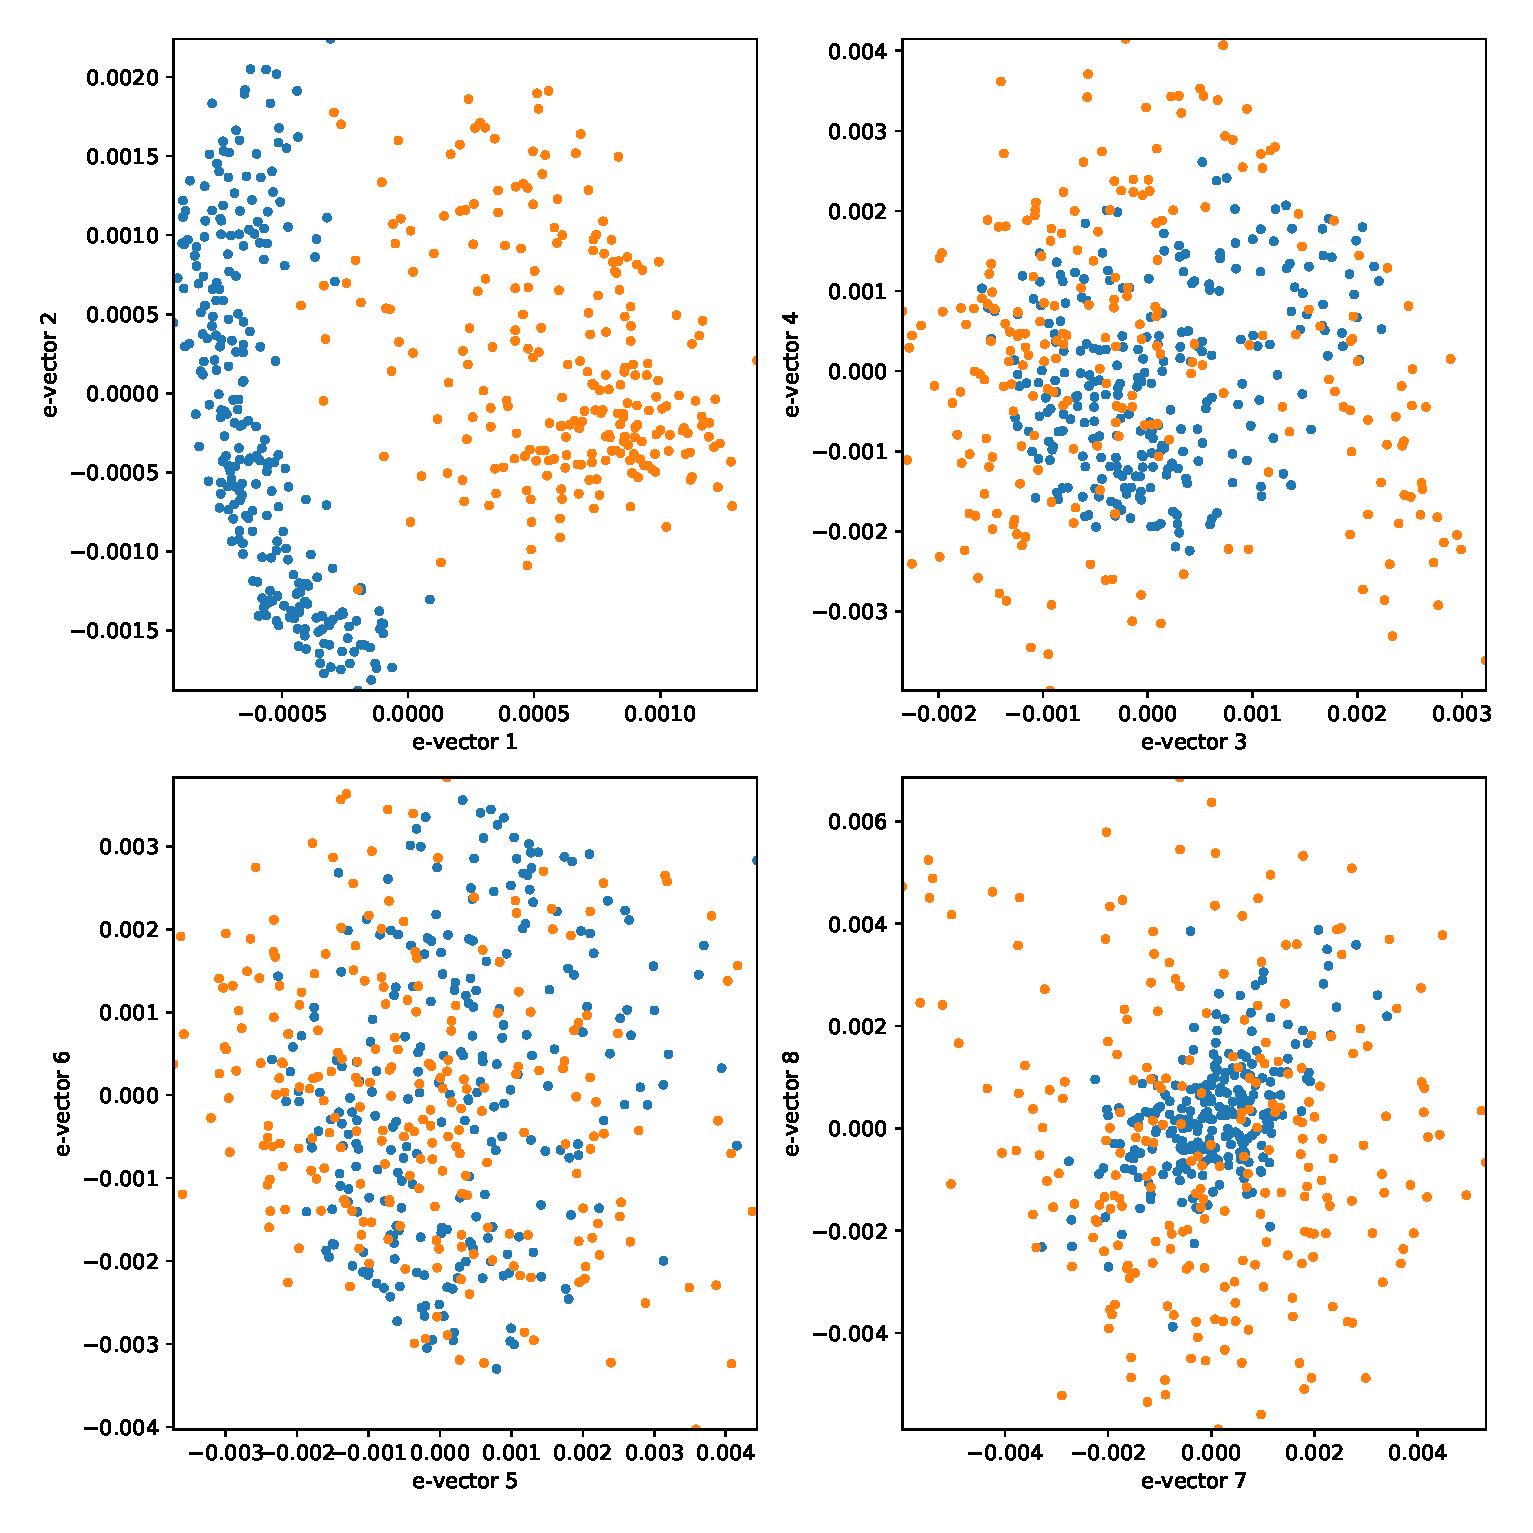
\includegraphics[width=0.8\textwidth]{./img/kpca_linear.eps}
\caption{\label{fig:kpca_lin}KPCA Using a Linear Kernel}
\end{figure}

\begin{figure}
	\centering 
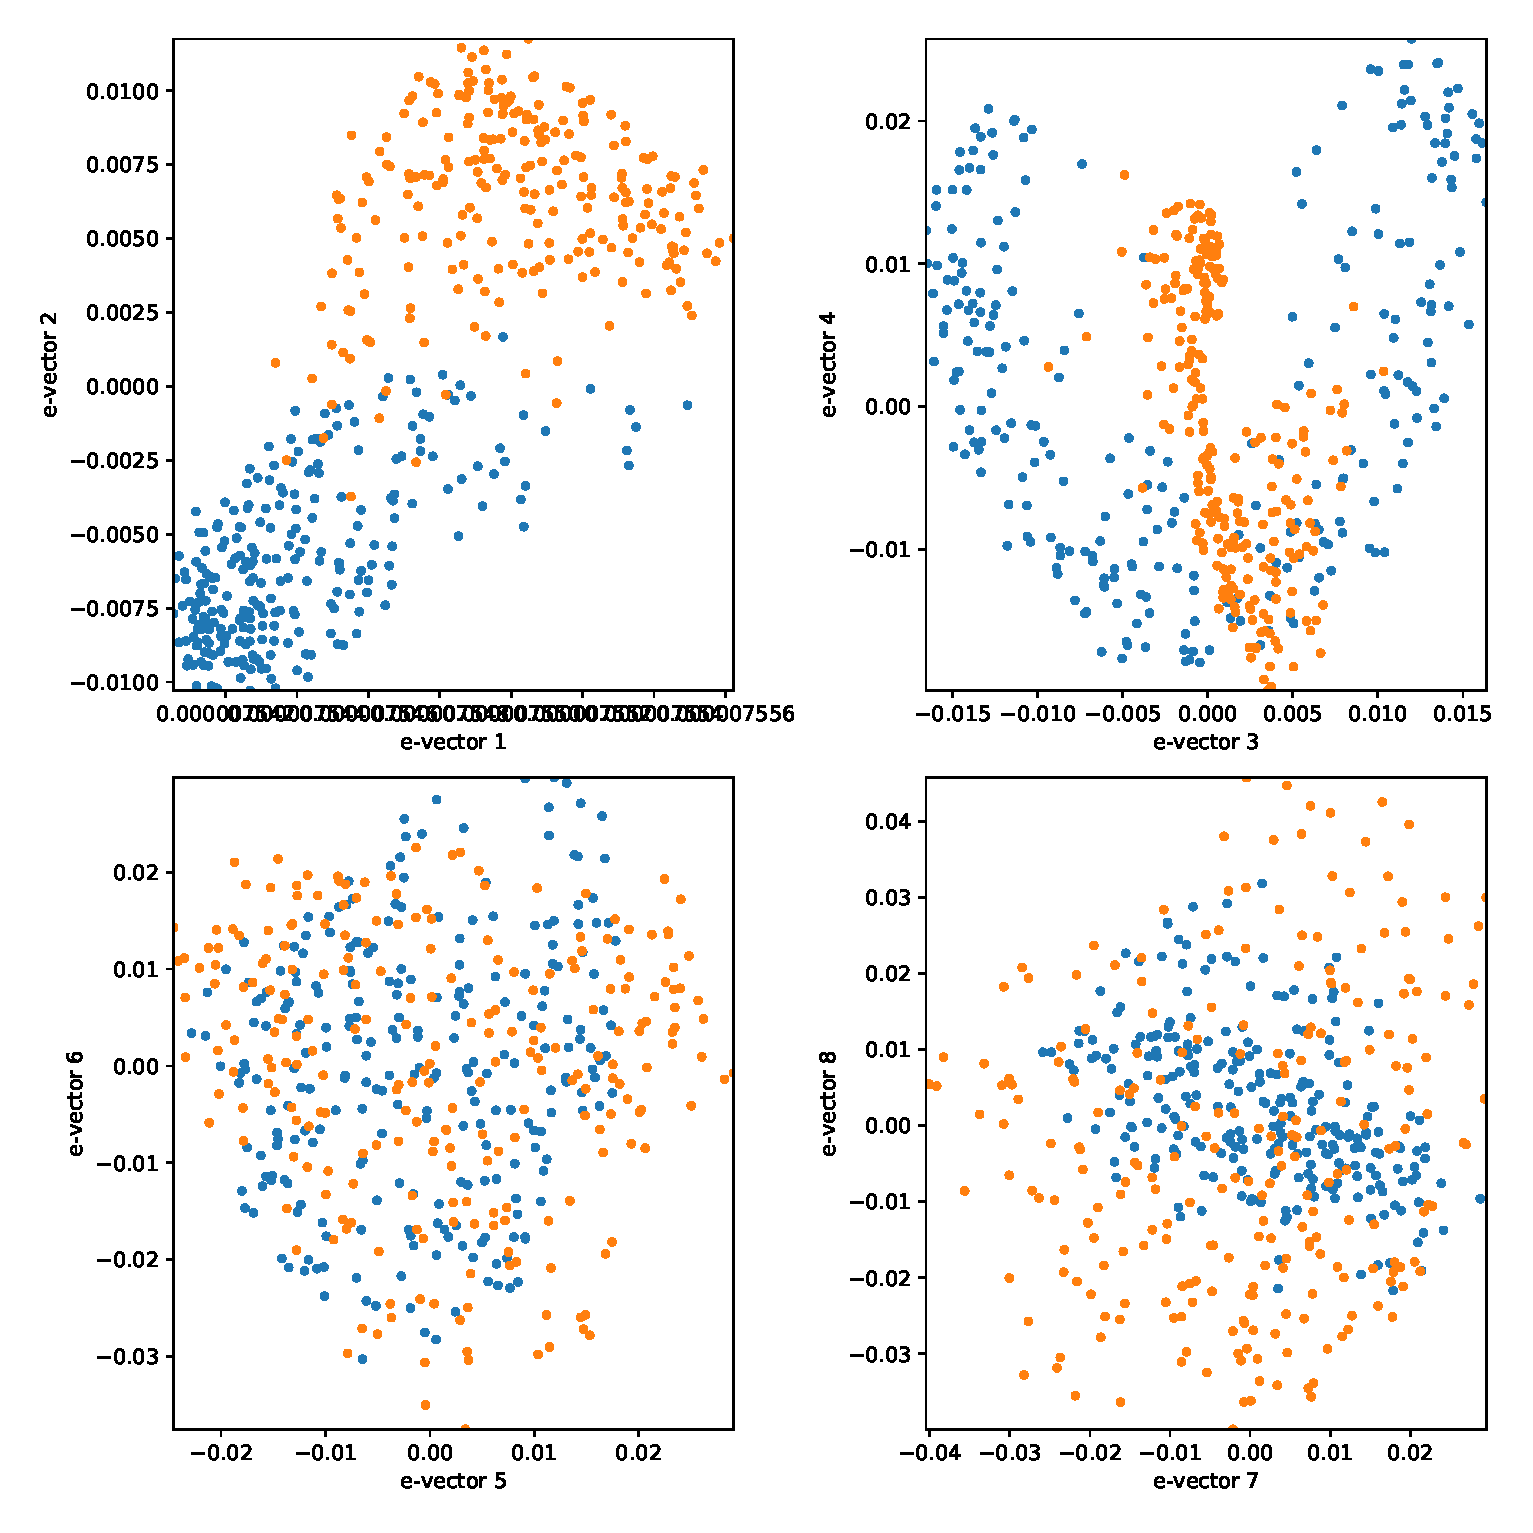
\includegraphics[width=0.8\textwidth]{./img/kpca_gaussian_5.eps}
\caption{\label{fig:kpca_gauss}KPCA Using a Gaussian Kernel ($\tau = 5$)}
\end{figure}


\begin{figure}
	\centering
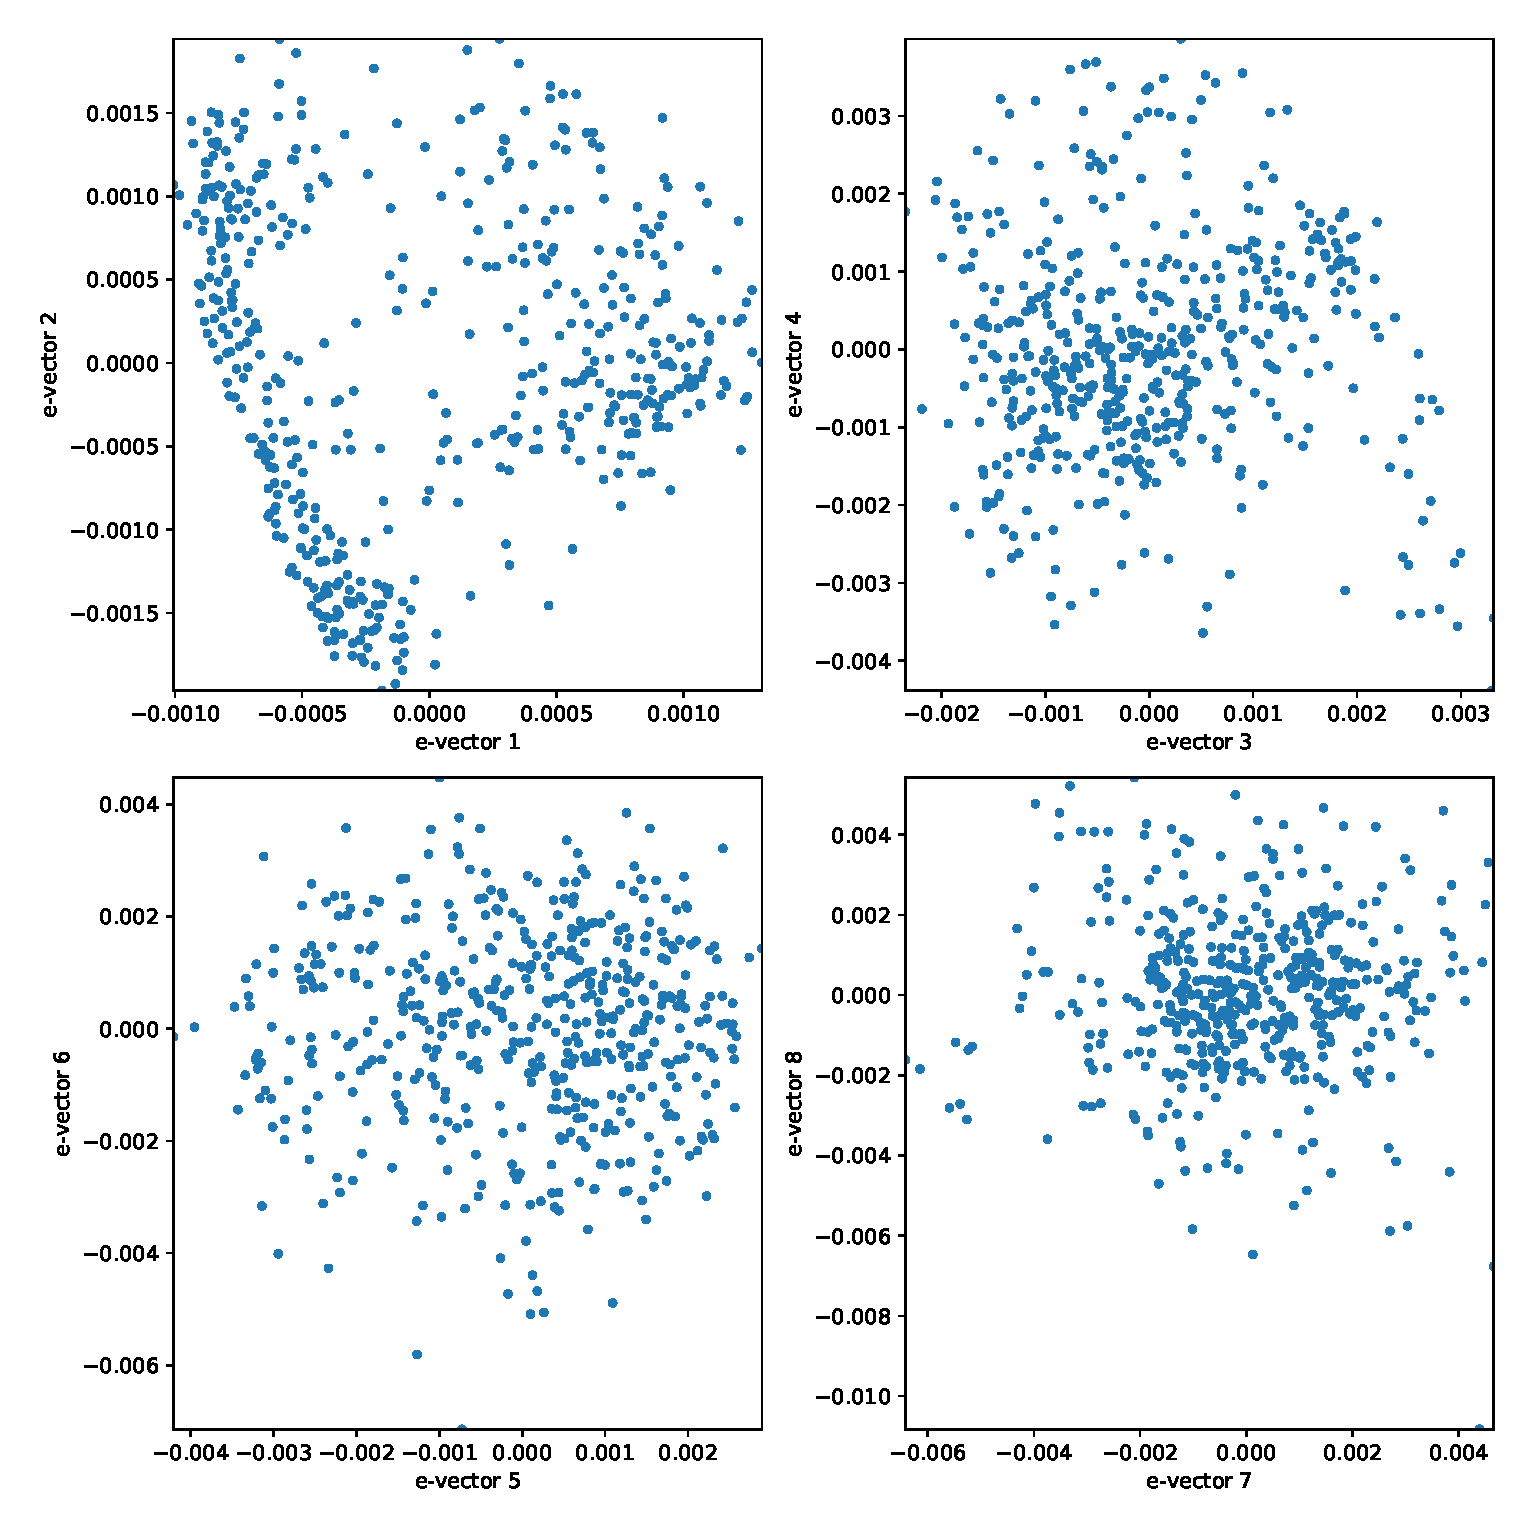
\includegraphics[width=0.8\textwidth]{./img/kpca_polynomial_3.eps}
\caption{\label{fig:kpca_poly}KPCA Using a Polynomial Kernel ($d=3$)}
\end{figure}

%\begin{figure}
%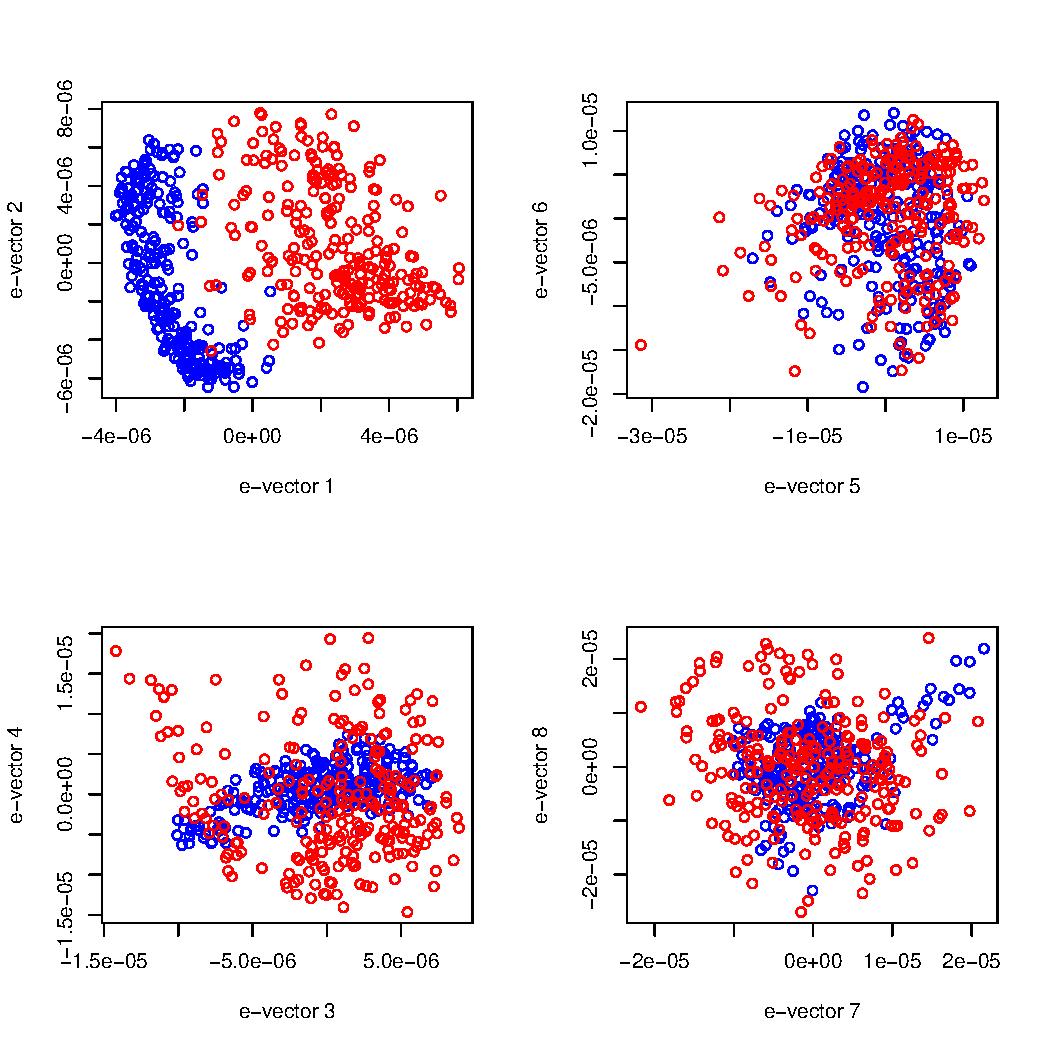
\includegraphics[width=0.8\textwidth]{kpca-mnist-linear.pdf}
%\caption{\label{fig:kpca}Example of resu;ts with Kernel PCA}
%\end{figure}
\end{enumerate}
\end{document}
